\documentclass{beamer}

%%%%%%%%%%%%%Solarized Theme%%%%%%%%%%%%%%%
\usecolortheme[dark,accent=cyan]{solarized}
\beamertemplatenavigationsymbolsempty
%%%%%Packages%%%%%
\usefonttheme{serif}
\usepackage[T1]{fontenc}
\usepackage[utf8]{inputenc}
\usepackage[english]{babel}

% \usepackage{fontspec}
% \setmainfont{Helvetica Neue}
\usepackage{minted}

\definecolor{DarkGray}{gray}{0.1}
\usemintedstyle{paraiso-dark}


\usepackage{graphicx}
\usepackage{hyperref}
\usepackage{colortbl, xcolor}
\usepackage{booktabs}
\usepackage{amsmath,amsthm, amssymb, latexsym}

\usepackage{tikz}
\usepackage{standalone}
\usepackage{siunitx}
\usetikzlibrary{calc, positioning, arrows, arrows.meta, shapes}

\begin{document}

\begin{frame}
    \begin{center}
        \LARGE{\textcolor{orange}{THE FALLACY OF MERITOCRACY}} \\

        \vspace{1.5cm}
        \normalsize{PyCon Balkan}

        \vspace{1cm}
        \normalsize{@NikoletaGlyn}

    \end{center}
\end{frame}

\begin{frame}
    \begin{center}
    
\includegraphics[width=0.24\textwidth]{static/cardiff_uni_logo.png}\hspace{6pt}
    
\includegraphics[width=0.24\textwidth, height=0.245\textwidth]{static/django_girls.png}\vspace{10pt}

    
\includegraphics[width=0.24\textwidth]{static/ssi-logo.png} \hspace{6pt}
    
\includegraphics[width=0.24\textwidth]{static/plos-logo.jpg}

    \end{center}
\end{frame}

\begin{frame}
    \begin{center}
    
\includegraphics[width=0.24\textwidth]{static/shake.png} \hspace{6pt}
    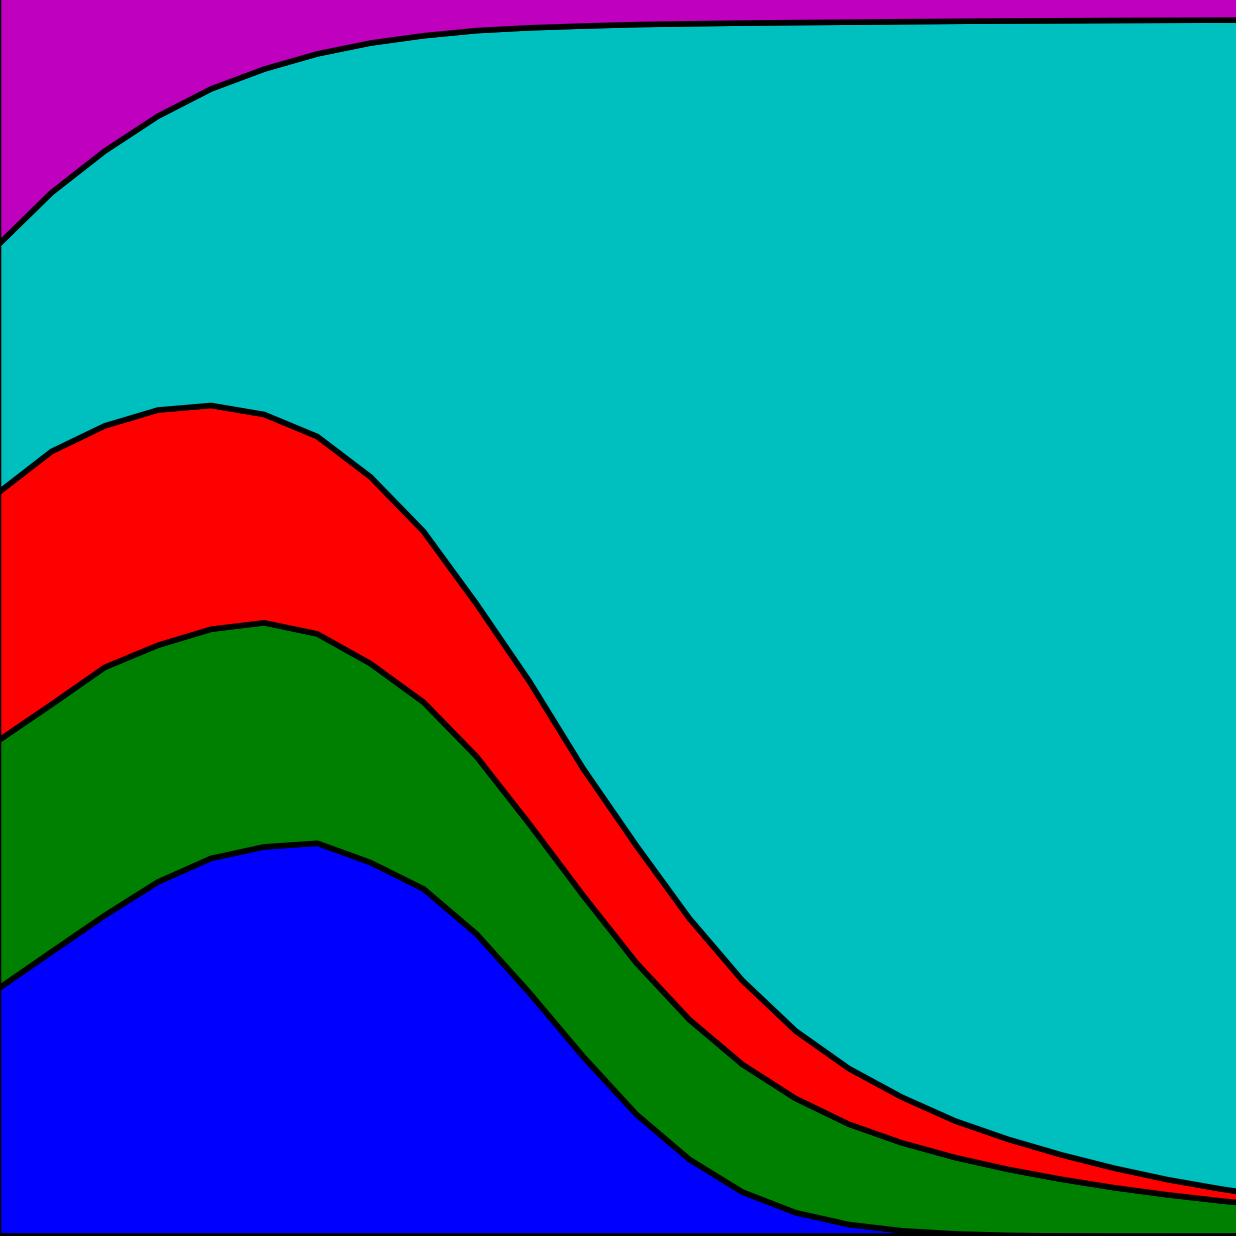
\includegraphics[width=0.24\textwidth]{static/axelrod-logo.png}

    \end{center}
\end{frame}

\begin{frame}
    \begin{center}
    \begin{minipage}{.5\textwidth}
        \LARGE{MERITOCRACY}
    \end{minipage}
    \begin{minipage}{.3\textwidth}
        \normalsize{[mer-i-tok-ruh-see]}
    \end{minipage}
    \vspace{.5cm}

    \hspace{-8cm} \normalsize{[noun]}\\
    \end{center}
    \hspace{.8cm} \normalsize{1. government or the holding of power by people}

    \hspace{1cm}\normalsize{selected according to merit.}
\end{frame}

\begin{frame}
    \begin{center}
    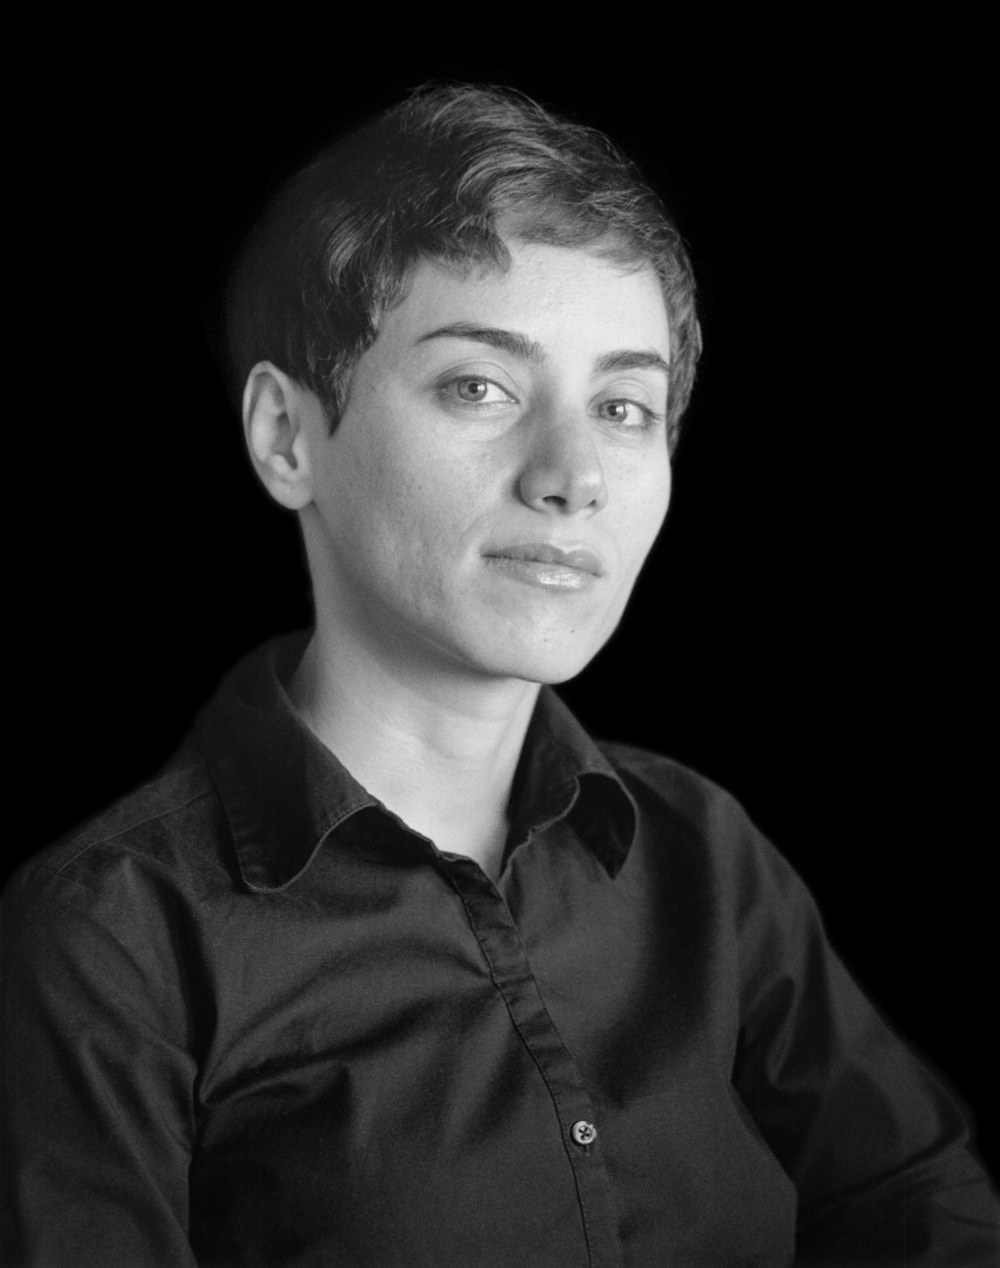
\includegraphics[width=0.4\textwidth]{static/maryam.jpg} \\
    \vspace{.8cm}
    \tiny{\url{www.newyorker.com/tech/annals-of-technology/maryam-mirzakhanis-pioneering-mathematical-legacy}}

    \end{center}
\end{frame}

\begin{frame}
    \begin{center}
    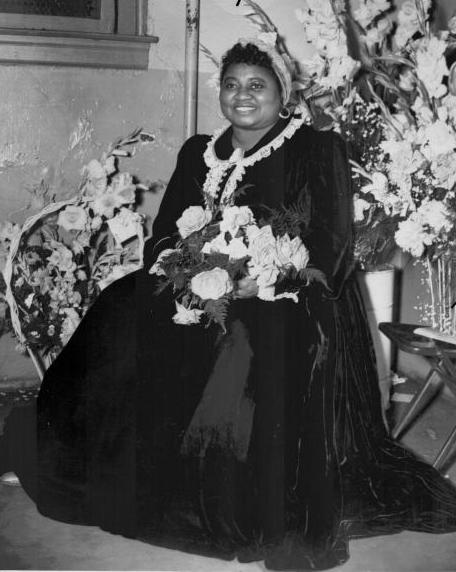
\includegraphics[width=0.40\textwidth]{static/hattie.jpg} \hspace{10pt}
    
\includegraphics[width=0.40\textwidth, height=.505\textwidth]{static/ali.jpg}
    \vspace{.8cm}
    \tiny{\url{en.wikipedia.org/wiki/List_of_black_Academy_Award_winners_and_nominees} \url{www.eonline.com/news/836150/}}

    \end{center}
\end{frame}

\begin{frame}
    \centering
    \LARGE \textbf{EQUALITY} \textcolor{orange}{VS} \textbf{EQUITY}
\end{frame}

\begin{frame}
    \begin{center}
    \begin{minipage}{.5\textwidth}
        \LARGE{EQUALITY}
    \end{minipage}
    \begin{minipage}{.3\textwidth}
        \normalsize{[ih-kwol-i-tee]}
    \end{minipage}
    \vspace{.5cm}

    \hspace{-8cm} \normalsize{[noun]}\\
    \end{center}
    \hspace{.8cm} \normalsize{1. the state of being equal, especially in status, or}

    \hspace{.8cm} \normalsize{opportunities.}
    \vspace{.5cm}

    \begin{center}
    \begin{minipage}{.5\textwidth}
        \LARGE{EQUITY}
    \end{minipage}
    \begin{minipage}{.3\textwidth}
        \normalsize{[ek-wi-tee]}
    \end{minipage}
    \vspace{.5cm}

    \hspace{-8cm} \normalsize{[noun]}\\
    \end{center}
    \hspace{.8cm} \normalsize{1.  the quality of being fair and impartial.} \\ 
\end{frame}

\begin{frame}
    \begin{center}
        \includestandalone[width=.45\textwidth]{static/race}
    \end{center}
\end{frame}

\begin{frame}
    \begin{center}
        \includestandalone[width=.45\textwidth]{static/race_equity}
    \end{center}
\end{frame}

\begin{frame}
    \begin{center}
    \begin{minipage}{.5\textwidth}
        \LARGE{BIAS}
    \end{minipage}
    \begin{minipage}{.3\textwidth}
        \normalsize{[bahy-uhs]}
    \end{minipage}
    \vspace{.5cm}

    \hspace{-8cm} \normalsize{[noun]}\\
    \end{center}
    \hspace{.8cm} \normalsize{1. a particular tendency, trend, inclination, feeling,}

    \hspace{1cm} \normalsize{or opinion, especially one that is preconceived or}

    \hspace{1cm} \normalsize{unreasoned.}
\end{frame}

\begin{frame}
    \begin{center}
        \textbf{\Large{TYPES OF \textcolor{orange}{UNCONSCIOUS} BIAS}} \\
        \hspace{1cm}

        \begin{minipage}{0.50\textwidth}
        \begin{itemize}
            \item Affinity Bias
            \item Halo Effect
            \item Horns Effect
            \item Attribution Bias
            \item Confirmation Bias
        \end{itemize}
        \end{minipage}
    \end{center}
\end{frame}

\begin{frame}
    \begin{center}
    \begin{minipage}{.5\textwidth}
        \LARGE{HOMOPHILY}
    \end{minipage}
    \begin{minipage}{.3\textwidth}
        \normalsize{[huh-mof-uh-lee]}
    \end{minipage}
    \vspace{.5cm}

    \hspace{-8cm} \normalsize{[noun]}\\
    \end{center}
    \hspace{.8cm} \normalsize{1. the tendency for people to seek out  those who are}

    \hspace{.8cm} \normalsize{similar to themselves.} \\
\end{frame}

\begin{frame}[fragile]
    \begin{minipage}{0.53\textwidth}
        \includestandalone[width=\textwidth]{static/states}
    \end{minipage}
    \begin{minipage}{0.42\textwidth}
        \vspace{-2.5cm}
        \begin{minted}
            [
            autogobble=true,
            framesep=2mm,
            fontsize=\tiny,
            bgcolor=DarkGray,
            ]
            {python}
>>> import hierarchy as hrcy
>>> capacities = [3, 2, 1]
>>> list(
... hrcy.states.get_states(capacities)
... )
[((0, 3), (0, 2), (1, 0)),
 ((0, 3), (1, 1), (1, 0)),
 ((0, 3), (2, 0), (1, 0)),
 ((0, 3), (0, 1), (1, 0)),
 ((0, 3), (1, 0), (1, 0)),
 ((1, 2), (0, 2), (1, 0)),
 ((1, 2), (1, 1), (1, 0)),
 ...
]
        \end{minted}
    \end{minipage}
\end{frame}

\begin{frame}
    \centering
    \hspace{-3.5cm}\LARGE{\textbf{\textcolor{orange}{RETIREMENT}}} \\
    \vspace{1cm}
    \begin{minipage}{0.41\textwidth}
        \includestandalone[width=\textwidth]{static/states}
    \end{minipage}\hspace{1cm}
    \begin{minipage}{0.41\textwidth}
        \includestandalone[width=\textwidth]{static/retirement_states}
    \end{minipage}
\end{frame}

\begin{frame}
    \centering
    \hspace{-3.5cm}\LARGE{\textbf{\textcolor{orange}{PROMOTION}}} \\
    \vspace{1cm}
    \begin{minipage}{0.41\textwidth}
        \includestandalone[width=\textwidth]{static/retirement_states}
    \end{minipage}\hspace{1cm}
    \begin{minipage}{0.41\textwidth}
        \includestandalone[width=\textwidth]{static/promotion_states}
    \end{minipage}
\end{frame}

\begin{frame}
    \centering
    \hspace{-3.5cm}\LARGE{\textbf{\textcolor{orange}{HIRING}}} \\
    \vspace{1cm}
    \begin{minipage}{0.41\textwidth}
        \includestandalone[width=\textwidth]{static/promotion_states}
    \end{minipage}\hspace{1cm}
    \begin{minipage}{0.41\textwidth}
        \includestandalone[width=\textwidth]{static/hire_states}
    \end{minipage}
\end{frame}

\begin{frame}[fragile]
    \begin{center}
        \begin{minted}
            [
            autogobble=true,
            framesep=2mm,
            fontsize=\scriptsize,
            bgcolor=DarkGray,
            ]
            {python}
>>> capacities = [3, 2, 1]
>>> state = [[2, 1],
...          [1, 1],
...          [1, 0]]
>>> potential_sts = hrcy.transitions.get_potential_states(state,
...                                                       capacities)
        \end{minted}
\pause
\begin{minted}
    [
    autogobble=true,
    framesep=3mm,
    fontsize=\scriptsize,
    bgcolor=DarkGray,
    ]
    {python}
>>> r = 1.1
>>> lmbda = [2, 3]
>>> mu = [[0.2, 0.1],
...       [1.2, 1.1],
...       [1.5, 1.7]]
>>> transitions = hrcy.transitions.get_transition_matrix(capacities,
...                                                      r,
...                                                      lmbda,
...                                                      mu)
\end{minted}
    \end{center}
\end{frame}

\begin{frame}
    \Large
    \begin{itemize}
        \item \(\mu_{ij}\)
        \item \(\text{max}(rs_{ij} + s_{i, \bar j}, 1)\)
        \item \(\lambda_{j}\)
    \end{itemize}
\end{frame}

\begin{frame}
    \Huge
    \begin{equation*}
        \bar{s} M = \bar{s}
    \end{equation*}
\end{frame}

\begin{frame}
    \centering
    \LARGE \textbf{COMPETENCE}
\end{frame}

\begin{frame}
    \centering
    \LARGE \textbf{UNCONSCIOUS \textcolor{orange}{BIAS}} \\
    \vspace{1cm}

    \LARGE \textbf{\textcolor{orange}{HOMOPHILY} EFFECT}
\end{frame}

\begin{frame}
    \Huge
    \begin{equation*}
        \bar{s} M = \bar{s}
        \end{equation*}
\end{frame}

\begin{frame}[fragile]
    \begin{minipage}{0.55\textwidth}
        \includestandalone[width=\textwidth]{static/competence}
    \end{minipage}
    \begin{minipage}{0.41\textwidth}
        \vspace{-2.5cm}
        \begin{minted}
            [
            autogobble=true,
            framesep=2mm,
            fontsize=\tiny,
            bgcolor=DarkGray,
            ]
            {python}
>>> import hierarchy as hrcy
>>> capacities = [3, 2, 1]
>>>
>>>
>>>
>>>
        \end{minted}
    \end{minipage}
\end{frame}

\begin{frame}
    \centering
    \LARGE \textbf{BE \textcolor{orange}{AWARE} OF YOUR UNCONSCIOUS BIAS}
\end{frame}

\begin{frame}
    \centering
    \LARGE \textbf{BE \textcolor{orange}{AN ALLY}}
\end{frame}

\begin{frame}
    \centering
    \LARGE \textbf{DO \textcolor{orange}{NOT} BE LAZY}
\end{frame}

\begin{frame}
    @NikoletaGlyn \\
    @drvinceknight
\end{frame}

\end{document}

